\documentclass[]{article}

% accenti
\usepackage[utf8]{inputenc}
% rimuove indentatura
\usepackage[parfill]{parskip}
% colori
\usepackage{color}
% per cambiare i margini della pagina
\usepackage{vmargin}
% per fissare le figure
\usepackage{float}

\usepackage{graphicx}
\begin{document}

\title{Grafi}
\author{Federico Magnolfi}
\maketitle

\section{Introduzione}
Si vuole analizzare l'algoritmo per trovare le componenti fortemente connesse in grafi diretti.

\section{Descrizione}
Un grafo G è composto da un insieme V di elementi detti nodi (o vertici) e da un insieme E di archi, ogni elemento di E è una coppia di elementi distinti di V. Il grafo si dice orientato (o diretto) se ogni arco ha una precisa direzione, ovvero se la coppia di vertici è ordinata.

Il numero di vertici è uguale alla cardinalità dell'insieme $V$ ($|V|$), il numero di archi è uguale alla cardinalità dell'insieme $E$ ($|E|$).

Si dice cammino tra due nodi $s$ e $d$, una sequenza $<v_0, v_1, ..., v_k>$ di vertici t.c. $s=v_0$, $d=v_k$ e $(v_{i-1},v_i)\in E$ per i = 1, ..., k

In un grafo non orientato, un insieme di vertici è connesso se ogni coppia di vertici è collegata attraverso un cammino.

In un grafo orientato, un insieme di vertici è fortemente connesso se ogni coppia di vertici è collegata attraverso un cammino in entrambe le direzioni.

Le componenti connesse di un grafo non orientato, e le componenti fortemente connesse di un grafo orientato, sono classi di equivalenza dei vertici secondo la relazione "è raggiungibile da". Indichiamo una componente fortemente connessa con l'acronimo SCC(Strongly-Connected Component).

Dato un grafo $G = (V, E)$, il suo trasposto è $G^T = (V, E^T)$, ovvero un altro grafo avente lo stesso insieme V di vertici, e con gli archi invertiti.

Preso un nodo sorgente $s\in V$, la visita di G consiste nell'elencare tutti i vertici del grafo a partire da $s$ secondo una determinata strategia. In particolare trattiamo la visita in profondità (Depth-First Search, DFS), che esplora prima i nodi raggiungibili dal nodo $s$, e poi il nodo stesso, ricorsivamente, creando un albero di nodi raggiungibili da $s$. Si itera il procedimento prendendo come nodo $s$ un altro nodo che ancora non è stato visitato: alla fine si ha una foresta di alberi, dove ogni nodo è sicuramente raggiungibile dai propri antenati, inoltre la foresta prodotta non è univoca. Per eseguire la DFS, si memorizzano nei nodi i seguenti attributi:

\begin{itemize}
\item id: numero che identifica il nodo
\item color: colore del nodo, serve per sapere se è già stato visitato o meno
\item p: predecessore del nodo, quello da cui discende nell'albero
\item d: tempo di scoperta del nodo
\item f: tempo di fine esplorazione del sotto-albero del nodo
\end{itemize}

L'algoritmo che cerca le componenti fortemente connesse di un grafo orientato $G$ si bassa sulla DFS, che inizialmente viene eseguita su G. Dopodiché calcola $G^T$ e chiama la DFS su di esso, con la particolarità che i nodi $s$ non vengono presi a caso, ma in ordine decrescente rispetto al campo $f$ calcolato con la prima DFS. Ogni albero della foresta generata dalla seconda DFS, è una componente fortemente connessa di G (e anche di $G^T$).

\section{Analisi teorica}
Un grafo può essere rappresentato in più modi, uno di questi è attraverso la matrice di adiacenza: è una matrice di dimensione $|V|*|V|$, in cui l'elemento sulla riga $i$ e colonna $j$ è 1 se (i, j) $\in E$, altrimenti è 0. Con questa rappresentazione, il grafo trasposto può essere facilmente ottenuto eseguendo la trasposta della matrice di adiacenza.

La rappresentazione tramite matrice di adiacenza permette inoltre di poter generare grafi casuali in modo semplice: assegnata una certa probabilità $p$, ogni elemento della matrice (arco) sarà 1 con probabilità $p$, 0 con probabilità $1-p$.

Si vogliono analizzare il numero di archi, il numero di SCC ed il tempo di esecuzione dell'algoritmo che cerca le SCC su grafi casuali, al crescere del numero di nodi e della probabilità $p$ di generazione degli archi.

Il numero di archi sarà compreso tra 0 $|V|*|V|$, si vuole verificare che sia proporzionale alla probabilità di generazione degli archi.

Ci si aspetta che il numero di SCC decresca all'aumentare di $p$, e che diventi 1 (tutto il grafo è fortemente connesso) oltre una certa soglia. Quando $p$ è 0, il numero di SCC sarà uguale a $|V|$.

Quanto al tempo di esecuzione dell'algoritmo, si vede che dipende dal tempo di esecuzione delle 2 DFS, dal tempo di calcolo della trasposta. Ogni DFS esplora sempre ogni arco e nodo del grafo ed ha quindi un costo temporale di $\Theta(|V|+|E|)$. Il tempo per ottenere la trasposta dipenderà dall'implementazione nella libreria usata, ma sarà sicuramente inferiore a quello della DFS. Non viene misurato il tempo che sarebbe necessario per trovare il dettaglio dei nodi che compongono le SCC.

\section{Descrizione esperimenti}
Si generano grafi casuali con numero di nodi e probabilità di generazione archi differenti.
Il numero di nodi che si testano sono tutti i numeri compresi tra 1 e 99 (inclusi, solo numeri dispari). Per ogni numero di nodi, si testano tutte le probabilità comprese nell'intervallo [0, 1) con passo 0.01.

Per ogni combinazione di numero di nodi e probabilità, si eseguono 10 test durante i quali si calcola la media del numero di archi, del numero di SCC e del tempo di esecuzione dell'algoritmo. I valori calcolati vengono salvati su un file csv, e vengono alla fine mostrati in tre grafici tridimensionali: in funzione di probabilità (asse x) e numero nodi (asse y) vengono mostrati i valori corrispondenti (asse z) di numero di archi (primo grafico), numero di SCC (secondo grafico) o tempo di esecuzione (terzo grafico).

\subsection*{Piattaforma di test}
Il test viene eseguito su un computer desktop con le seguenti caratteristiche:
\begin{itemize}
\item Sistema Operativo: Linux Mint 18.1
\item CPU: Intel Core i5-2400 (6 MB cache, 3.40 Ghz)
\item RAM: 16 GB
\item linguaggio di programmazione e interprete: Python 3.5
\item IDE: PyCharm 2017
\end{itemize}

\section{Documentazione del codice}
Il programma è composto da 2 file: grafocasuale.py, exp.py.

\subsection*{grafocasuale.py}
Implementa le funzioni utili all'utilizzo dei grafi e alla generazione di grafi casuali. Contiene 3 classi:
\begin{itemize}

\item Node: classe che gestisce un nodo, presenta i seguenti attributi:
\begin{itemize}
\item id: numero che identifica il nodo
\item color: colore del nodo, serve per sapere se è già stato visitato o meno
\item p: predecessore del nodo, quello da cui discende nell'albero
\item d: tempo di scoperta del nodo
\item f: tempo di fine esplorazione del sotto-albero del nodo
\end{itemize}

\item Graph: classe che gestisce un grafo, presenta i seguenti attributi e metodi:
\begin{itemize}
\item adjMatrix: matrice di adiacenza del grafo, oggetto di tipo ndarray con valori booleani
\item nodes: lista di nodi del grafo, con valori di tipo Node
\item time: numero intero che tiene traccia del tempo, utile durante la DFS
\item \_\_init\_\_(adjMatrix=None, numNodes=0): costruttore che crea il grafo tramite la matrice di adiacenza se specificata, altrimenti ne crea una vuota (piena di 0) della dimensione indicata.
\item dfs(firstGraph=None): esegue la DFS, ovvero richiama la dfsVisit su tutti i nodi che non sono stati ancora visitati. Il parametro eventuale è un grafo su cui è già stata effettuata la DFS e serve per sapere l'ordine in cui prendere i nodi su cui chiamare la dfsVisit. Se non specificato, i nodi vengono considerati in ordine di id. Ritorna il numero di alberi nella foresta esplorata.
\item dfsVisit(nodeId): esegue la visita a partire dal nodo avente l'id indicato. Chiama sé stessa ricorsivamente sui nodi raggiungibili dal nodo id, colorando i nodi e modificando gli attributi d, f e p durante la visita.
\item transpose(): ritorna il grafo trasposto di sé stesso.
\item getNumStronglyConnectedComponents(): ricerca il numero di componenti fortemente connesse nel grafo, implementando l'algoritmo descritto in precedenza, senza tuttavia cercare il dettaglio dei nodi che le compongono. Ritorna il numero di componenti fortemente connesse.
\item getStronglyConnectedComponents(): ricerca le componenti fortemente connesse nel grafo, implementando l'algoritmo descritto in precedenza. Ritorna una lista di componenti fortemente connesse, dove ognuna di esse è la lista di nodi che le appartengono.
\end{itemize}

\item RandomGraph(Graph): classe che estende Graph, viene ridefinito il costruttore:
\begin{itemize}
\item \_\_init\_\_(numNodes, prob): genera un grafo casuale con numero di nodi e probabilità di generazione archi indicati.
\end{itemize}

\end{itemize}

\subsection*{exp.py}
È formata da una funzione di test e dal programma principale:
\begin{itemize}
\item test(n, p, points): genera 10 grafi casuali aventi $n$ nodi e $p$ probabilità di generare archi, calcolando numero medio di SCC e tempo di esecuzione. Aggiunge alla lista points un elemento formato nel seguente modo: 
\begin{verbatim}
[p, n, avgNumEdges, avgNumSCC, avgExecTime]
\end{verbatim}
questo sarà poi utile per salvare su file csv i risultati degli esperimenti. Ritorna i due valori calcolati.
\item main(): inizializza due vettori di tipo ndarray contenenti probabilità e numero di nodi da testare. Utilizzando funzioni della libreria numpy, si esegue il test per ogni possibile combinazione di probabilità e numero nodi. Si salvano i risultati sul file "data.csv" e si creano i tre grafici tridimensionali.
\end{itemize}

\section{Risultati sperimentali}

I risultati ottenuti nella fase di test sono riportati nel file "data.csv". Con i risultati ottenuti, vengono realizzati tre grafici tridimensionali che vengono riportati sotto.

\begin{center}
\begin{figure}[H]
	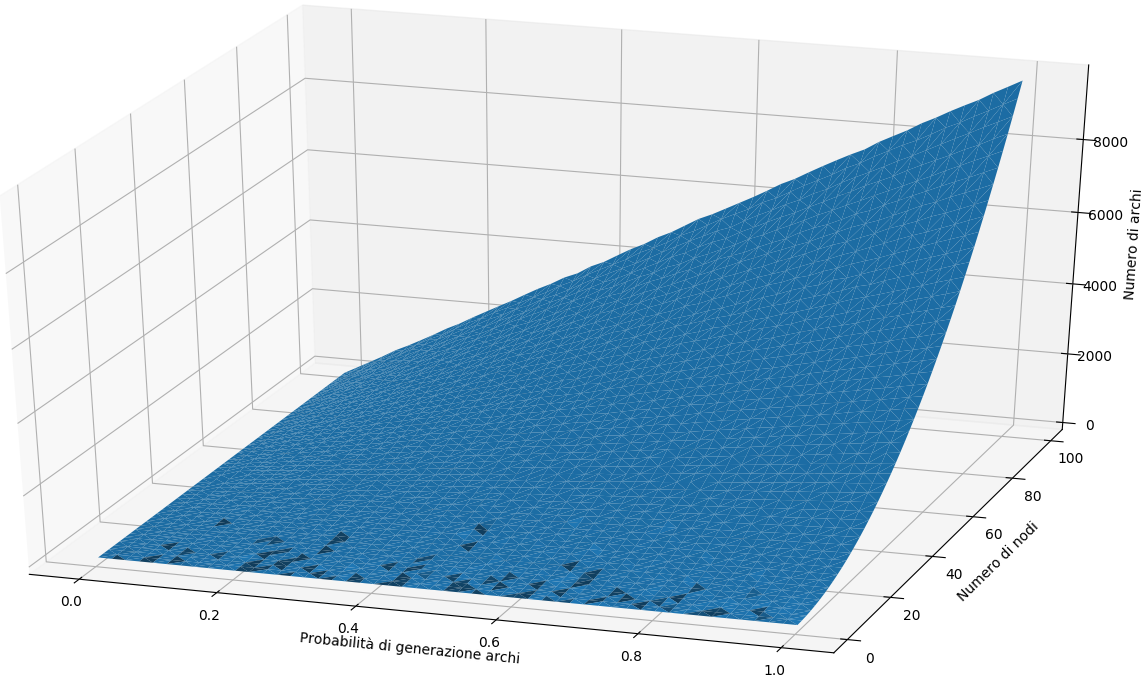
\includegraphics[width=\linewidth]{grafici/numEdges.png}
	\caption{Numero medio di archi misurato su 10 test, in funzione di numero di nodi e probabilità generazione archi.}
	\label{imgNumeroArchi}
\end{figure}
\end{center}

\begin{center}
\begin{figure}[H]
	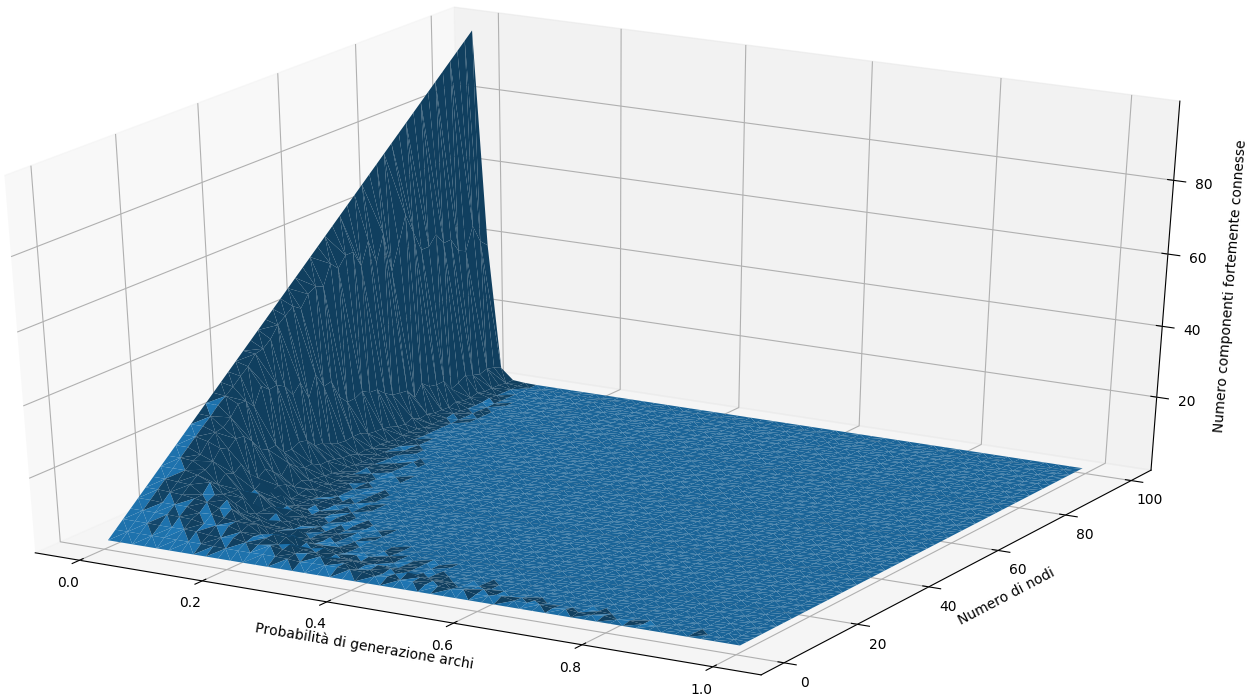
\includegraphics[width=\linewidth]{grafici/numSCC.png}
	\caption{Numero medio di componenti fortemente connesse misurate in 10 test, in funzione di numero di nodi e probabilità generazione archi.}
	\label{imgNumeroSCC}
\end{figure}
\end{center}

\begin{center}
\begin{figure}[H]
	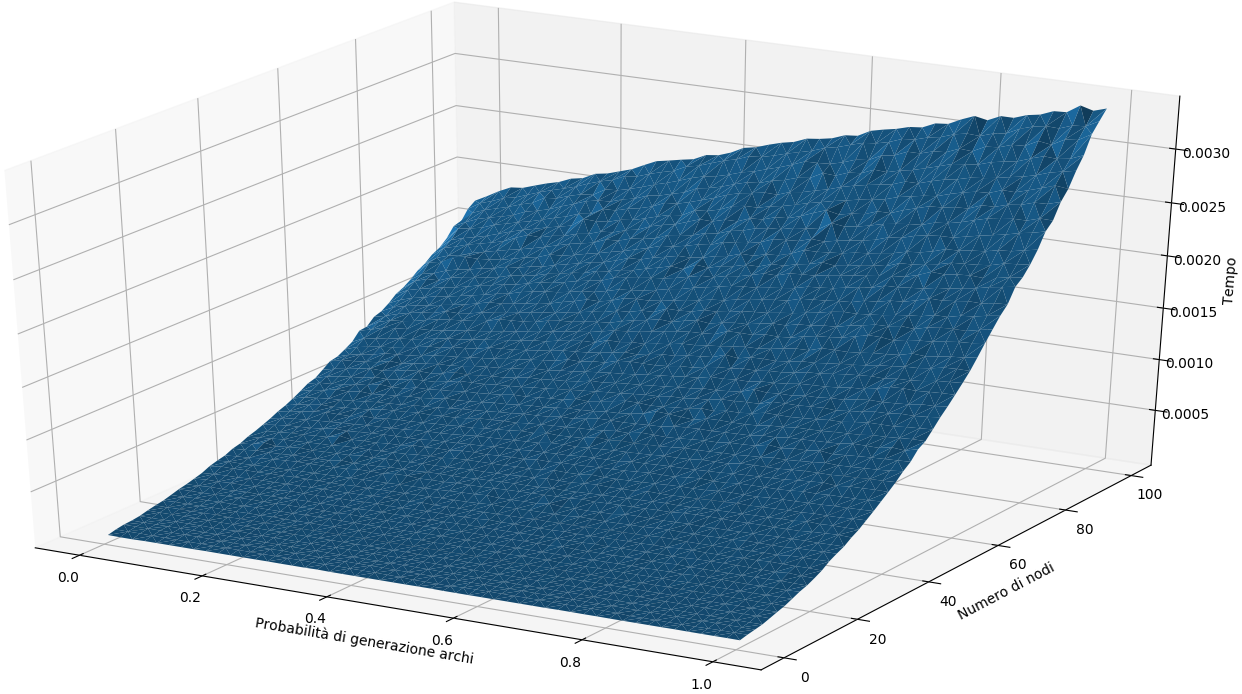
\includegraphics[width=\linewidth]{grafici/execTimes.png}
	\caption{Tempi medi di esecuzione su 10 test dell'algoritmo che cerca il numero di componenti fortemente connesse, in funzione di numero di nodi e probabilità generazione archi.}
	\label{imgTempiEsecuzione}
\end{figure}
\end{center}


\section{Analisi dei risultati}
Come si nota dal primo grafico, il numero di archi è effettivamente proporzionale alla probabilità di generazione degli archi.

Il numero di SCC decresce all'aumentare di $p$, e diventi 1 (tutto il grafo è fortemente connesso) oltre una certa soglia, che è tanto più bassa più sono i nodi. Quando $p$ è 0, il numero di SCC è uguale a $|V|$.

Il tempo di esecuzione dell'algoritmo è $\Theta(|V|+|E|)$. Infatti, fissato un numero di nodi e considerando che il numero di archi varia proporzionalmente alla probabilità, dal grafico si vede (sezione sullo sfondo a destra) che il tempo aumenta in modo lineare, a partire da una quota iniziale.

\section{Conclusioni}
Gli esiti degli esperimenti sono compatibili con ciò che era stato previsto.
L'algoritmo che ricerca componenti connesse nei grafi ha un tempo di esecuzione asintotico $\Theta(|V|+|E|)$.


\end{document}